\documentclass{article}

\usepackage[T1,T2A]{fontenc}
\usepackage[utf8]{inputenc}
\usepackage[english]{babel}
\usepackage{xcolor}
\usepackage{booktabs}
\usepackage{amsfonts}
\usepackage{algorithm}
\usepackage{algorithmicx}
\usepackage{algpseudocode}
\usepackage{amstext}
\usepackage{hyperref}
\usepackage{amssymb}
\usepackage{amsmath}
\usepackage{chemfig}
\usepackage{wrapfig}
\usepackage{subcaption}
\usepackage{tikz}

\usetikzlibrary{trees}

\bibliographystyle{apalike}

% aliases
\newcommand{\F}{\mathcal{F}}
\newcommand{\M}{\mathcal{M}}
\newcommand{\T}{\mathbb{T}}

\DeclareMathOperator*{\argmax}{arg\,max}
\DeclareMathOperator*{\argmin}{arg\,min}

\title{Substructure search optimizations}

\begin{document}
\maketitle

%\input{Introduction}
\section{Introduction}
Substructure search in chemical compound databases is a vital task in cheminformatics, underpinning broad applications in drug discovery, 
materials science, and toxicology. The objective is to identify all molecules in a database that contain a given query substructure, which 
typically corresponds to a specific chemical motif or functional group. This search has been a cornerstone in understanding the influence 
of specific substructures on a compound's biological activity, physicochemical properties, and reactivity, a recognized concept for 
decades \cite{barnard1993}.

Historically, computer-based substructure search started with pioneers like Ledley and colleagues who developed the Chemical Substructure 
Search (CSS) algorithm in the 1960s and 1970s \cite{ledley1964}. This algorithm employed a graph-based approach to identify specific 
substructures in chemical compounds. Further advancements in the field came with the development of the Simplified Molecular Input 
Line Entry System (SMILES) notation by Weininger in the 1980s \cite{weininger1988}, which provided a simple, linear representation 
of molecular structures as strings.

Substructure search fundamentally rests on the solution of the subgraph isomorphism problem, a problem known to be NP-complete \cite{ullmann1976}. 
Due to its high computational complexity, numerous heuristics and algorithms have been devised to accelerate the search process. 
Among these, the Filter-and-Verification paradigm has been a prevalent approach, involving an initial filtering step to quickly 
eliminate unsuitable candidate graphs, and a more computationally intensive verification step to confirm the presence of the query 
substructure in the remaining candidates \cite{cordella2004, shasha2002}. Over time, graph-based subgraph isomorphism algorithms, 
such as the Ullmann algorithm \cite{ullmann1976} and the VF2 algorithm \cite{cordella2004}, have emerged as more efficient and 
scalable solutions for substructure search in large chemical databases.

In addition to these, frequent subgraph mining algorithms like gSpan \cite{yan2002}, FFSM \cite{kuramochi2001}, and Gaston \cite{nijssen2004} 
have proven valuable in identifying frequently occurring substructures in large sets of chemical compounds. These approaches 
are particularly beneficial for applications such as structure-activity relationship (SAR) analysis and molecular classification.

Efficient filtering techniques often involve the use of binary and quantitative features, or fingerprints, to represent molecular 
structures. These fingerprints facilitate the rapid elimination of graphs that do not contain specific features required by the 
query subgraph, thereby speeding up the substructure search process \cite{bonchi2011, klein2014}.

However, as the number of known molecules and the size of chemical databases have grown exponentially, the traditional approaches, 
which often require full or nearly full enumeration of candidates, have become increasingly challenging to implement efficiently. 
This development underlines the need for more scalable solutions.

{\color{red} Информация про экспоненциальный рост взята из обсуждений с коллегами проекта. Однако, я не могу сослаться на авторитетный источник, подтверждающий экспоненциальный рост. Поэтому предлагаю написать более аккуратно. Например, сказать, что у компании есть датасет размера 4 миллиарда, и что текущие подходы не позволяют эффективно поддерживать такую большую базу данных. Поэтому и есть потребность в поиске нового алгоритма. (А где-то в итогах можно упомянуть, что наш подход в текущей версии всё ещё не решает задачу для 4 миллиардов) }

Our work presents a novel approach that addresses these limitations by moving beyond the conventional full enumeration paradigm. 
{\color{red} в худшем случае наше решение выполняет полный перебор, поэтому не уверен, можно ли тут сказать, что мы вышли за его рамки} 
Instead, we introduce a unique index structure: a tree that segments the molecular dataset into clusters based on the presence or 
absence of features. Inspired by the binary Ball-Tree concept \cite{omohundro1989, clarkson1994}, this structure demonstrates 
superior performance over exhaustive search on average, leading to a significant acceleration in the filtering process.

We provide a comparative analysis of our method with Sachem {\color{red} \cite{Kratochvil2018}}, a known fast search method, highlighting key differences. While Sachem 
uses advanced filtering effectively, it relies on exhaustive search in a chemical space that continually expands. In contrast, 
our approach departs from exhaustive search and places an existing molecular fingerprint into a tree structure, rather than a 
conventional relational database. While the current version of our approach does not significantly speed up the verification 
stage
{\color{red} Но ведь текущая версия абсолютно не влияет на verification stage. Поэтому у нас абсолютно нет улучшений части verification}, the potential lies in reducing the false positive rate and enhancing the verification process runtime.
{\color{red} в предыдущем абзаце мне было бы непонятно, что уже реализовано, а что только появиться быть в нашей будущей версии. }
By introducing this innovative structure, we aim to cater to the growing scale of chemical databases and the escalating demand 
for efficient and scalable search solutions. Our approach offers potential for future research and application in the quest 
for more efficient and accurate substructure search techniques.


\begin{figure}
\centering

\resizebox{!}{0.8\totalheight}	
{
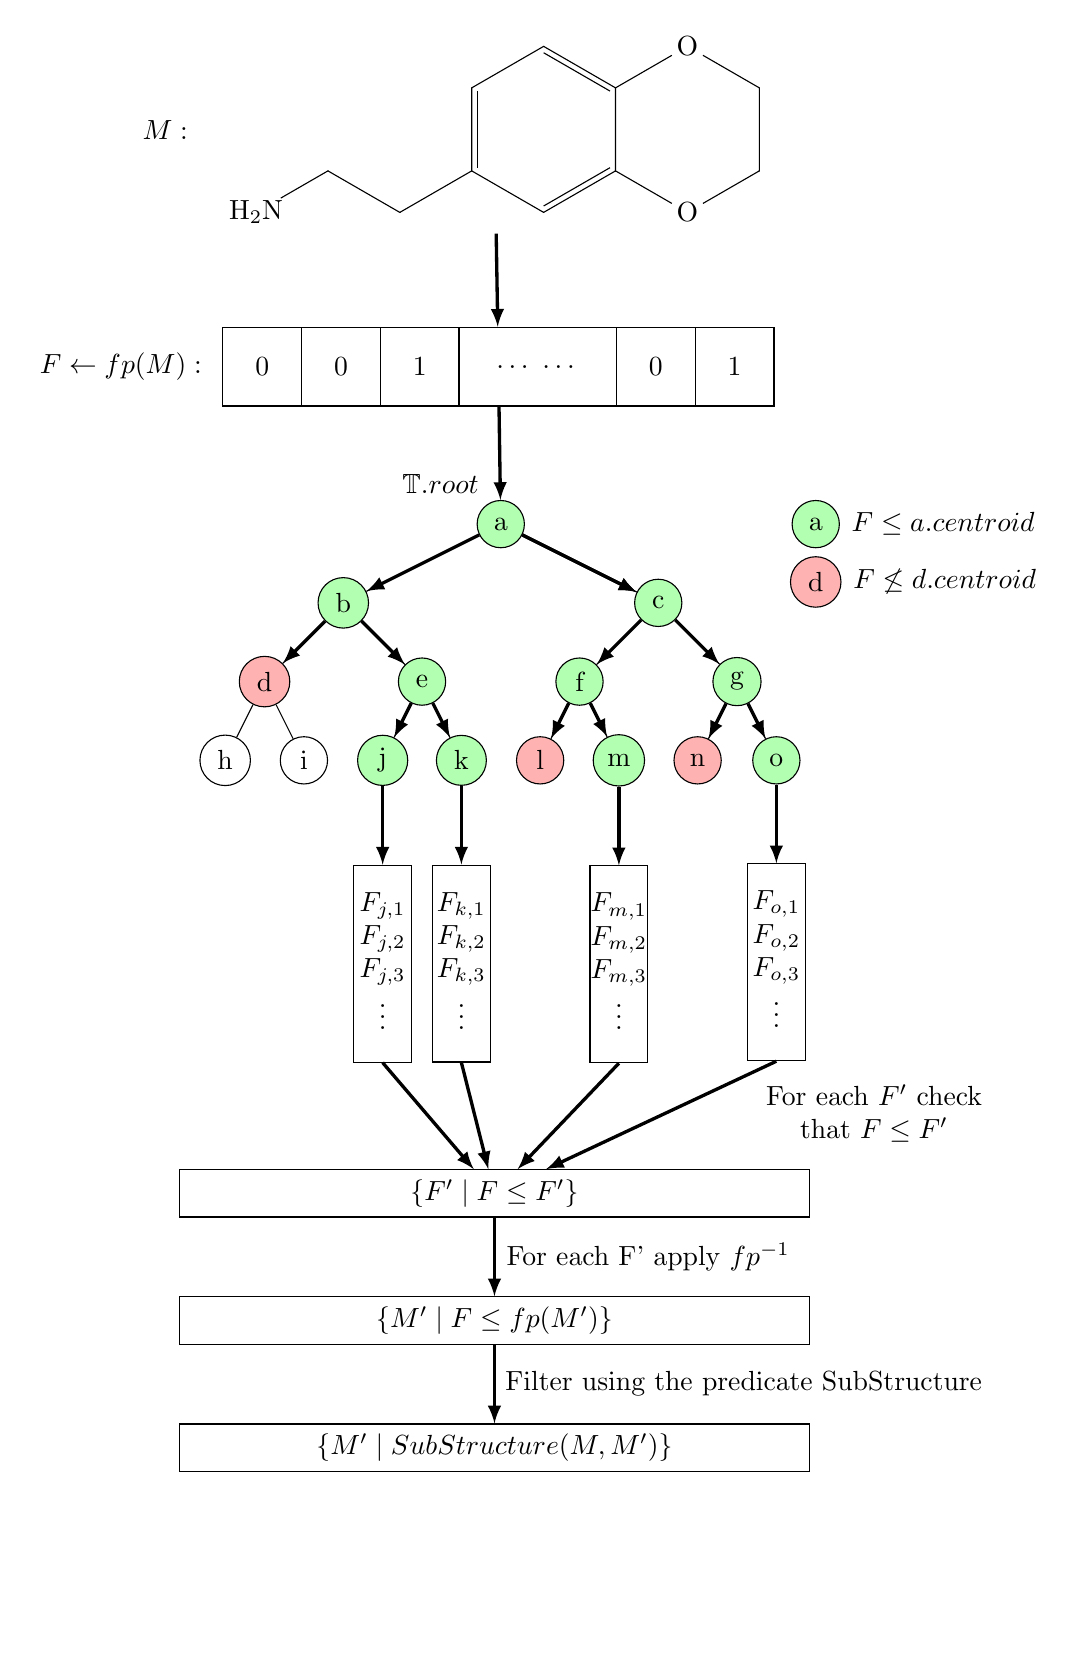
\begin{tikzpicture}[level distance=1cm,
  level 1/.style={sibling distance=4cm},
  level 2/.style={sibling distance=2cm},
  level 3/.style={sibling distance=1cm},
  every node/.style={circle,draw,minimum size=.6cm},
  bucket/.style={draw,rectangle,minimum height=2.5cm, text width=.5cm,align=center},
  stop_node/.style={fill=red!30},
  continue_node/.style={fill=green!30},
  arrow/.style={-latex,very thick},
  text_box/.style={rectangle,minimum width=8cm},
  fp_cell/.style={rectangle,draw,minimum width=1cm,minimum height=1cm},
  ]
  \usetikzlibrary{positioning}

  % molecule
  \node[name=molecule,rectangle,draw=none, minimum width=8cm]
  {
    \chemfig[angle increment=30,bond join=true]{
	*6(
	(
	-[-5]-[5]-
	{H_2N}
	)
	-=
	*6(
	-
	O
	---
	O
	-
	)
	-=-=
	)
    } 
  };

  % fingerprint
  \begin{scope}[yshift=-3cm,xshift=-2.95cm, minimum width=8cm]
    \node(fingerprint)[fp_cell,draw=none] at (3, 0) {};
    \node[fp_cell] at (0,0) {0};
    \node[fp_cell] at (1,0) {0};
    \node[fp_cell] at (2,0) {1};
    \node[fp_cell,minimum width=3cm] at (4,0) {  };
    \node[draw=none] at (3.5,0) {$\dots \ \dots$};
    \node[fp_cell] at (5,0) {0};
    \node[fp_cell] at (6,0) {1};
  \end{scope}

  % tree
  \begin{scope}[yshift=-5cm,xshift=0.08cm]
    \node[name=a,continue_node,label=170:{$\T.root$}] {a}
    child {node[name=b,continue_node]  {b}
      child {node[name=d,stop_node] {d}
	child {node[name=h] {h}}
	child {node[name=i] {i}}
      }
      child {node[name=e,continue_node] {e}
	child {node[name=j,continue_node] {j}}
	child {node[name=k,continue_node] {k}}
      }
    }
    child {node[name=c,continue_node] {c}
      child {node[name=f,continue_node] {f}
	child {node[name=l,stop_node] {l}}
	child {node[name=m,continue_node] {m}}
      }
      child {node[name=g,continue_node] {g}
	child {node[name=n,stop_node] {n}}
	child {node[name=o,continue_node] {o}}
      }
    };

    \begin{scope}[xshift=4cm,node distance=.1cm]
      \node (legend_a) [continue_node,label=right:{$F \le a.centroid$}] {a}; 
      \node (legend_d) [stop_node,below=of legend_a,label=right:{$F \not\le d.centroid$}] {d}; 
    \end{scope}
   
    \foreach \i in {j, k, m, o} {
      \node[name=bucket_\i,bucket,below=of \i]  {};
      \node[draw=none] at (bucket_\i.center) {
	  \begin{tabular}{c}
	    $F_{\i,1}$ \\
	    $F_{\i,2}$ \\
	    $F_{\i,3}$ \\
	    $\vdots$ 
	  \end{tabular} 
	};
    }
  \end{scope}
 
  % text boxes
  \begin{scope}[yshift=-13.5cm,node distance=1cm] 
    \node (filtered_fingerprints) [text_box]
      {
	$\{F' \mid F \le F'\}$ 
      };

  \foreach \i in {bucket_j, bucket_k, bucket_m}
    \draw[arrow] (\i.south) -- (filtered_fingerprints);


  \node (compounds) [text_box,below=of filtered_fingerprints]
    {
      $\{M' \mid F \le fp(M')\}$ 
    };
  
  \node (filtered_compounds) [text_box,below=of compounds]
    {
      $\{M' \mid SubStructure(M, M')\}$ 
    };
  \end{scope}

  % Arrows 
  \draw[arrow] (molecule) -- (fingerprint);
  \draw[arrow] (fingerprint) -- (a);  
  \foreach \from/\to in {a/b, b/d, e/j, c/f, f/l, g/n, a/c, b/e, e/k, a/c, c/g, g/o, f/m}
    \draw[arrow] (\from) -- (\to);

  \foreach \from/\to in {j/bucket_j, k/bucket_k, m/bucket_m, o/bucket_o}
    \draw[arrow] (\from) -- (\to);
  \draw[arrow] (bucket_o.south) -- (filtered_fingerprints) 
    node[draw=none,right,midway,xshift=9mm] 
    {
      \begin{tabular}{c}
	For each $F'$ check \\
	that $F \le F'$ 
      \end{tabular}
    };

  \draw[arrow] (filtered_fingerprints) -- (compounds)
    node[draw=none,right,midway]
    {
      For each F' apply $fp^{-1}$ 
    };

  \draw[arrow] (compounds) -- (filtered_compounds)
    node[draw=none,right,midway]
    {
      Filter using the predicate SubStructure 
    };
  
  % Labels
  \node[left=of molecule,draw=none,xshift=1.3cm] {$M:$}; 
  \node[left=of fingerprint,draw=none,xshift=-2.1cm] {$F \gets fp(M):$}; 

\end{tikzpicture}
}
\end{figure}

\section{Algorithm description}

\subsection{Notation and main idea}
The objective of our research is to facilitate the identification of specific substructures within the molecules from a database $\M$. 
For this, we utilize the concept of a ``fingerprint'', a binary string of constant length ${\sf fl}$, corresponding to each molecule. 
To perform this mapping, we define a function ${\sf fp}: \M \to \F$ that takes a molecule from the set $\M$ and produces its 
corresponding fingerprint in the set $\F$. {\color{red} На мой взгляд написано слишком кратко про фингерпринты. Кажется, если 
человек не в теме, то он может не понять, что это за сопоставление молекулам бинарных строк, зачем оно нужно и почему оно эффективно реализует этап filter}

To make the substructure search process more efficient, we propose organizing these fingerprints in a binary search tree, denoted as $\T$. The tree is binary and complete, having a specific depth $d$.

In this tree, the root, left, and right subtrees of a node $\tt{v}$ are represented as $\T.\tt{root}$, $\tt{v.left}$, and $\tt{v.right}$, 
respectively. Each node also has a set of all leaves in its subtree, denoted as $\tt{v.leaves}$. Each leaf $\ell$ in the tree $\T$ holds 
a set $\ell.\tt{set}$ of fingerprints. A unique concept to our approach is the centroid, ${\tt v.centroid}$, recorded at each node $v$. 
The centroid is defined as a fingerprint $F$ for which $F[i] = 1$ if and only if there exists another fingerprint $F'$ in the subtree 
of $\tt{v}$ such that $F'[i] = 1$. This is represented as
$${\tt v.centroid} = \bigvee\limits_{\ell \in {\tt v.leaves}}\bigvee\limits_{F \in \ell.{\tt set}} F.$$ 
This concept of the centroid is inspired by BallTree literature.

Our search process is designed to locate all fingerprints $F'$ in the set $\F$ where $F$ is a submask of $F'$. This search relies on the relation $F_1 \le F_2$ for fingerprints $F_1, F_2$ that holds true if and only if for every $i \in {1, 2, \ldots, {\sf fl}}, \ F_1[i] \le F_2[i]$. 

The search starts from the root and recursively descends into both subtrees. Note that here we can improve the performance by parallelizing 
this step to explore both subtrees simultaneously. We stop the recursive descent if we reach a node ${\tt v}$ where $F \not\le {\tt v.centroid}$. 
Conversely, if we reach a leaf $\ell$ and $F \le \ell.{\tt centroid}$, we add to $\F_M$ the set $\{F' \in  \ell.{\tt set} \mid {\sf fp}(M) \le F'\}$.

Following the generation of $\F_M$, the next phase involves examining each $M'$ in $\bigcup\limits_{F' \in \F_M} {\sf fp}^{-1}(F')$. The 
objective is to determine whether each $M'$ is a substructure of $M$. This determination is made by employing external algorithms to verify the predicate $\verb|SubStructure|(M', M)$, which is true if and only if $M'$ is a substructure of $M$. 

Further details on the BallTree and the utilization of the tree in the substructure search process will be provided in the subsequent sections.



The pseudocode for the fingerprint search function in the tree is described in Algorithm \ref{alg:FindInSubtree}. The pseudocode for the function that searches for superstructures of a given molecule is described in Algorithm \ref{alg:FindMetaStructures}.

\begin{algorithm}[h!]
  \caption{Searching for all matching fingerprints in a subtree}\label{alg:FindInSubtree}
  \begin{algorithmic}[1]
    \Require{${\tt v}$ is a tree vertex, $F$ is a fingerprint}
    \Ensure{$\{F' \in \bigcup\limits_{\ell \in {\tt v.leaves}} \ell.{\tt set} \mid F \le F' \}$}
    \Procedure{FindInSubtree}{${\tt v}, F$} 
    \If{$F \not\le {\tt v.centroid}$} \label{alg:FindInSubtree:line:RecursionCut}
      \State \textbf{return} $\varnothing$
    \ElsIf{${\tt v} \text{ is leaf}$}
      \State \textbf{return} $\{F' \in {\tt v.set} \mid F \le F' \}$ 
    \Else
      \State ${\tt left} \gets $ \Call{FindInSubtree}{${\tt v.left}, F$}  
      \State ${\tt right} \gets $ \Call{FindInSubtree}{${\tt v.right}, F$} 
      \State \textbf{return} \Call{Concatenate}{${\tt left}, {\tt right}$} 
    \EndIf
    \EndProcedure
  \end{algorithmic}
\end{algorithm}

\begin{algorithm}[!ht]
  \caption{Searching for all superstructures of a given molecule} \label{alg:FindMetaStructures}
  \begin{algorithmic}[1]
    \Require $M $ is a molecule 
    \Ensure $\{M' \in \M \mid {\tt SubStructure}(M, M') \}$ 
    \Procedure{FindMetaStructures}{$M $}
    \State $F \gets {\sf fp}(M) $ 
    \State $F_M \gets $ \Call{FindInSubtree}{$\T.{\tt root}, F$}
    \State \textbf{return} $\{M' \in \bigcup\limits_{F' \in F_M} {\sf fp}^{-1}(F') \mid \Call{SubStructure}{M, M'}\}$ 
    \EndProcedure
  \end{algorithmic}
\end{algorithm}

\subsection{Building the tree}

\begin{algorithm}
  \caption{Building the tree} \label{alg:BuildTree}
  \begin{algorithmic}[1]
    \Require $\F$ is the set of all fingerprints, $d$ is the depth of the tree
    \Ensure $\T $ is the BallTree for the superstructure fingerprint search 
    \Procedure{BuildTree}{$\F, d$}
      \State ${\tt v} \gets$ new node
      \If{$d = 1$} 
      %\Comment{{\color{red} уточнить, остановка на $d = 1$ или на $d = 0$}} 
	\State ${\tt v.set} \gets \F$ 
	\State ${\tt v.centroid} \gets \bigvee\limits_{F \in \F} F$ 
	\State \textbf{return} ${\tt v}$ 
      \Else 
        \State $\F_l, \F_r \gets $ \Call{SplitFingerprints}{$\F$}
        \State ${\tt v.left} \gets $ \Call{BuildTree}{$\F_l, d - 1$} 
	\State ${\tt v.right} \gets $ \Call{BuildTree}{$\F_r, d - 1$}
	\State ${\tt v.centroid} \gets {\tt v.left.centroid} \lor {\tt v.right.centroid}$ 
        \State \textbf{return} ${\tt v}$ 
      \EndIf
    \EndProcedure
  \end{algorithmic}
\end{algorithm}

To start, let's create a trivial tree with a single node, denoted as $\T.{\tt root}$. Assign $\T.{\tt root.set} = \F$. 
Next, we will inductively split the leaves of the tree into two parts, thereby adding new nodes to the tree.

More formally, for each leaf node $\ell$ of the tree, we will divide $\ell.{\tt set}$ using a specific function called 
SplitFingerprints: $\F_l, \F_r \gets \text{SplitFingerprints}(\ell.{\tt set})$ ($\F_l \sqcup \F_r = \ell.{\tt set}$).
Next, we will recursively build trees for $\ell.{\tt left}, \ell.{\tt right}$ using the sets $\F_l, \F_r$.

We will continue splitting the leaves in this manner until $\T$ becomes a full binary tree with depth $d$. The pseudocode 
for the algorithm described above can be found in \ref{alg:BuildTree}.
 

\begin{algorithm}
  \caption{Algorithm for splitting fingerprints in parts during tree construction} \label{alg:SplitFingerprints}
  \begin{algorithmic}[1]
    \Require set $\F$ of fingerprints to be split
    \Ensure the split $\F_l, \F_r$ of the set $\F$
    \Procedure{SplitFingerprints}{$\F $}
      \State $j \gets \argmin\limits_{i}\{ \left| |\F| - 2k \right| \mid k = \# \{F \in \F \mid F_i = 1 \} \}$ %\Comment{{\color{red} стоит ли пояснить формулу?}}
      \State $\F_l \gets \{F \in \F \mid F[j] = 0\}$
      \State $\F_r \gets \{F \in \F \mid F[j] = 1\}$ 
      \If {$|\F_l| > \lfloor \frac{n}{2} \rfloor$}
	\State $\F_r \gets \F_r \ \cup$ \Call{TakeLastElements}{$\F_l, |\F_l| - \lfloor \frac{n}{2} \rfloor$}
	\State $\F_l \gets $ \Call{DropLastElements}{$\F_l, |\F_l| - \lfloor \frac{n}{2} \rfloor$} 
      \ElsIf{$|\F_r| > \lceil \frac{n}{2} \rceil$}
	\State $\F_l \gets \F_l \ \cup$ \Call{TakeLastElements}{$\F_r, |\F_r| - \lceil \frac{n}{2} \rceil$}
	\State $\F_r \gets $ \Call{DropLastElements}{$\F_r, |\F_r| - \lceil \frac{n}{2} \rceil $} 
      \EndIf
      \State \textbf{return} $\F_l, \ \F_r$ 
    \EndProcedure
  \end{algorithmic}
\end{algorithm}

We want to perform the splits in such a way that, on average, the search often prunes branches during the traversal. 
That is, the {\bf if} statement in line \ref{alg:FindInSubtree:line:RecursionCut} of algorithm \ref{alg:FindInSubtree} 
should be executed frequently. Let's discuss the function SplitFingerprints in more detail.

Initially, one might consider selecting a specific bit $j$ and assigning all fingerprints $F$ such that $F[j] = 0$ to 
the left subtree, and those with $F[j] = 1$ to the right subtree. In this case, when searching for superstructures of 
the fingerprint $F'$, if $F'[j] = 1$, the entire left subtree would be cropped. However, in practice, this approach leads 
to significant differences between the left and right parts after a few splits, making it difficult to create a deep and 
balanced tree. Unfortunately, a shallow or unbalanced tree does not offer substantial improvements over a full search, 
as it barely eliminates any search branches.

Therefore, we suggest the following method: we will still select the bit as mentioned above, but we will divide the 
fingerprints in a way that ensures the sizes of the resulting partitions match. For instance, if the optimal division 
of $n$ fingerprints yields parts with sizes $n_0, n_1 (n_0 < n_1 \ \land \ n_0 + n_1 = n)$, then all values with zero 
will be assigned to the left partition, while the values with one will be distributed to achieve final left and right 
partition sizes of $\lfloor\frac{n}{2}\rfloor, \lceil \frac{n}{2} \rceil$ respectively. If $n_0 > n_1$, we will proceed 
symmetrically. The algorithm for the SplitFingerprints function can be found in the pseudocode \ref{alg:SplitFingerprints}.

\section{Benchmarks}

In this study, we have carried out comprehensive benchmarking to assess the performance of our algorithm, which is an extension 
of the Bingo fingerprinting system, in comparison with established indices, namely Bingo {\color{red}\cite{Pavlov2010}} and Sachem/Lucy {\color{red} \cite{Kratochvil2018}}.
{\color{red} В Sachem статье есть ещё сравнения Sachem/OrChem, Sachem/eCDK, RDKit, pgchem. Можно их тоже перенести в бенчмарки чтобы база сравнений была шире.}
Our benchmarking process 
was performed under the following conditions:

\begin{itemize}
\item OS: Ubuntu 22.04
\item Processor: Intel Xeon E5-2686 v4 (Broadwell)
\item Clock speed: 2.7 GHz
\item RAM: 120 GB
\end{itemize}

The query dataset used for benchmarking was retrieved from \url{https://hg.sr.ht/~dalke/sqc/browse?rev=tip}, which contains 3488 
relevant queries for substructure search. Ten queries were excluded due to various issues, resulting in a final set of 3478 compounds.
{\color{red} Кажется, плохо так сильно обобщать проблемы. Мы выкинули те молекулы, на которых наш алгоритм работает заведомо плохо. Поэтому выкинув эти 10 молекул мы улучшили свои результаты. С другой стороны 10 штук почти не влияют на статистику, поэтому может и нет смысла описывать подробности}.

We believe that this comparison is appropriate because the Sachem search in the referenced study was conducted in a similar manner. 
However, there are some notable differences between our testing conditions and those of the referenced studies. Our testing was 
performed on a processor with a higher clock speed (2.7 GHz versus 2.6 GHz), the database used in our tests was larger (113M 
compared to 94M), and our search was conducted for the first 10,000 results.
{\color{red} Ещё одно отличие: Sachem выкинули 159 запросов из 3488.}

Despite these differences, the benchmark results provide a meaningful comparison of the relative efficiencies of the three systems. 
For a single-threaded in-memory execution
{\color{red} Надо либо добавить в сравнительную таблицу версию, работающую на жёстком диске, либо убрать приписку "in-memory", потому что без версии во внешней памяти она не имеет смысла. Однако, из-за возникших технических трудностей, на данный момент у меня нет качественно проделанных замеров версии с жёстким диском}
, our algorithm demonstrates competitive performance, and it also shows the potential for 
parallelization, exhibiting substantial improvements when executed on 16 threads in memory.

The table below summarizes these benchmark timings, providing a clear comparison between our algorithm, Bingo, and Sachem/Lucy.
{\color{red} Bingo и Sachem тестировались тоже с искусственным ограничением на один поток. О чём сделал приписку в таблице}

\begin{center}
\begin{tabular}{|c|c|c|c|c|}
    \hline
    \% & \begin{tabular}{@{}c@{}}Our Algorithm,\\ single-threaded\\ in-memory\end{tabular} (s) 
       & \begin{tabular}{@{}c@{}}Our Algorithm,\\ 16-threaded\\ in-memory\end{tabular} (s) 
       & \begin{tabular}{@{}c@{}}Bingo,\\single-threaded\end{tabular} (s)
       & \begin{tabular}{@{}c@{}}Sachem/Lucy,\\single-threaded\end{tabular} (s) \\
    \hline
    50\% & 2.17443 & 0.337058 & 1 & - \\
    60\% & 3.83995 & 0.525275 & - & - \\
    70\% & 4.87392 & 0.677609 & - & - \\
    80\% & 6.71327 & 0.895 & 10 & - \\
    85\% & - & - & - & 1 \\
    90\% & 12.9814 & 1.65519 & - & - \\
    95\% & 30.2751 & 3.75599 & 100 & 10 \\
    98\% & - & - & - & 10 \\
    100\% & - & - & - & $<$80 \\
    \hline
\end{tabular}
\end{center}

This thorough analysis offers valuable insights into the performance and potential scalability of our algorithm, especially when it comes to parallel computing.
{\color{red} мне не кажется, что способность к распараллеливанию является нашим преимуществом, так как другие подходы тоже умеют работать параллельно}

\section{Further Development}

Fingerprints currently form the basis of our algorithm, but they do have certain limitations which don't make them the ideal fit for our tree-based approach.

Firstly, the fingerprint's condensed nature is aimed to ensure efficient computation, which often leads to grouping together several characteristics. 
For instance, a single attribute in a fingerprint often encapsulates multiple individual elements because these isolated items, while lacking substantial 
filtering power across the entire dataset, might be relevant for specific subsets. However, the fingerprint structure doesn't account for such instances. 
Contrarily, our approach could accommodate more complex functions, even if they operate slower than traditional filtering methods—for example, using 
a fingerprint variant that doesn't amalgamate different elements.

Secondly, fingerprints are designed to provide a universal filter across the entire dataset. This results in a significantly pared-down set of 
attributes applicable to the entire database. For example, Bingo utilizes 2584 attributes, which intuitively seems insufficient to capture all 
peculiarities of a 113M-sized molecule dataset. Even a substantially enlarged fingerprint variant wouldn't be able to cover all exceptional cases. 
In contrast, our approach, by dealing with subsets, can extract a unique characteristic for a tree node relevant to the set in the given subtree, 
thus allowing for a much more effective coverage of the existing data nuances.

As a result, a potential enhancement of our algorithm might involve the use of a specific attribute in each tree node. Depending on its presence or absence, 
the search continues in both subtrees or only in the right subtree. This attribute would be chosen in advance to approximately bisect the set in the subtree. 
A leaf would contain several characteristics which would be examined when filtering elements from the leaf.

Employing the method described above, we could potentially improve the false positive rate, as the selected attributes would be relevant to the examined subsets. 
Moreover, these attributes could be utilized during verification, possibly resulting in substantial improvements in the verification stage speed, thanks to the 
relevance of these attributes to the molecule subsets.

\section{Conclusion}

The current version of our approach can serve as an extension to a fingerprint, enhancing the filtering speed by avoiding exhaustive enumeration. Moreover, 
the tree's ability to cluster molecules enables a more detailed examination of cluster-specific attributes, an aspect that existing algorithms struggle with, 
as they aim to find optimal ways to generalize across the entire dataset. Therefore, our approach could potentially be used in the future to improve both the 
false-positive rate and the verification speed.

%\section{References}

{\color{red} TODO}

\begin{itemize}
  \item {\color{red} Найти что-то про описание ball tree и метрику Rassel-Rao}
  \item {\color{red} Pubchem}
  \item {\color{red} Indigo fingerprint, RDKit fingerprint}
  \item {\color{red} Что-то про AWS}

\end{itemize}


\bibliography{biblio}

\end{document}
